\documentclass[aspectratio=169,10pt]{beamer}
\usetheme{Madrid}

\usepackage{fancybox,graphicx,hyperref,url}
\usepackage{tikz}
\usetikzlibrary{shapes,arrows}
\usetikzlibrary{positioning}
%\usepackage[T1]{fontenc}
\usepackage{booktabs}
\usepackage{enumitem}
\setbeamercovered{transparent}

\setlistdepth{9}
\setlist[itemize,1]{label=$\bullet$}
\setlist[itemize,2]{label=$\bullet$}
\setlist[itemize,3]{label=$\bullet$}
\setlist[itemize,4]{label=$\bullet$}
\setlist[itemize,5]{label=$\bullet$}
\setlist[itemize,6]{label=$\bullet$}
\setlist[itemize,7]{label=$\bullet$}
\setlist[itemize,8]{label=$\bullet$}
\setlist[itemize,9]{label=$\bullet$}
\renewlist{itemize}{itemize}{9}

\setlist[enumerate,1]{label=$\arabic*.$}
\setlist[enumerate,2]{label=$\alph*.$}
\setlist[enumerate,3]{label=$\roman*.$}
\setlist[enumerate,4]{label=$\arabic*.$}
\setlist[enumerate,5]{label=$\alpha*$}
\setlist[enumerate,6]{label=$\roman*.$}
\setlist[enumerate,7]{label=$\arabic*.$}
\setlist[enumerate,8]{label=$\alph*.$}
\setlist[enumerate,9]{label=$\roman*.$}
\renewlist{enumerate}{enumerate}{9}

\AtBeginSection[]{
  \begin{frame}[noframenumbering]
  \vfill
  \centering
  \begin{beamercolorbox}[sep=8pt,center,shadow=true,rounded=true]{title}
    \usebeamerfont{title}\insertsectionhead\par%
  \end{beamercolorbox}
  \vfill
  \end{frame}
}

\title[Verified Time-Aware Stream Processing]{Verified Time-Aware Stream Processing}

\author[Rafael Castro]{
  Rafael Castro G. Silva\\\medskip
  {\small \url{rafaelcgs10@gmail.com}}}

\date{02/11/2023}

\institute[UCPH]{
  Department of Computer Science \\
  University of Copenhagen}

\begin{document}

\begin{frame}
  \titlepage

\end{frame}

\begin{frame}[fragile]
  \frametitle{What is this PhD about?}
  \begin{columns}
    \begin{column}{0.45\textwidth}
      \begin{itemize}
        \item Distributed Systems
              \begin{itemize}
                \item Stream processing frameworks
                      \begin{itemize}
                        \item Dataflow models
                              \begin{itemize}
                                \item Timely Dataflow
                              \end{itemize}
                      \end{itemize}
              \end{itemize}
        \item Formal Methods
              \begin{itemize}
                \item Verification using proof assistants
                      \begin{itemize}
                        \item Isabelle proofs
                              \begin{itemize}
                                \item Verified and executable code
                              \end{itemize}
                      \end{itemize}
              \end{itemize}
      \end{itemize}
    \end{column}
    \begin{column}{0.55\textwidth}
    \end{column}
  \end{columns}
\end{frame}

\begin{frame}{Contents}
  \begin{itemize}
    \item Timely Dataflow
    \item Progress Tracking
    \item Verified Progress Tracking
    \item Verified Timely Dataflow
    \item Questions, comments and suggestions
  \end{itemize}
\end{frame}

\section{Timely Dataflow}

\begin{frame}[fragile, noframenumbering]
  \frametitle{Example of a conventional Dataflow}
  \begin{center}
    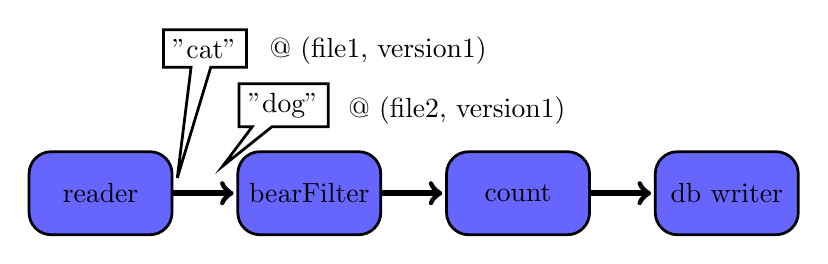
\begin{tikzpicture}[node distance = 0.8cm, auto]
\usetikzlibrary{shapes,arrows}
\usetikzlibrary{positioning}

\tikzstyle{operator} = [rectangle, draw, fill=blue!60, text width=4.5em, text centered, rounded corners = 8pt, minimum height=30pt, line width=1pt]
\tikzstyle{callout} = [draw, rectangle callout, callout relative pointer={#1}, line width=1pt]

    \node [operator] at (0, 0) (reader) {reader};
    \node [operator, right = of reader] (filter) {bearFilter};
    \node [operator, right = of filter] (count) {count};
    \node [operator, right = of count] (writer) {db writer};

    \draw [thick,->,shorten >=1pt, line width=2pt] (reader) -- (filter) 
       node[callout={(-0.3,-40pt)}, midway,above = 45pt] {"cat"} node[midway,above= 45pt, shift={(2.2,-0.1)}] {@ (file1, version1)}
       node[callout={(-0.5,-0.5)}, midway,above= 15pt, shift={(1.0,0.3)}] {"dog"} node[midway,above= 15pt, shift={(3.2,0.2)}] {@ (file2, version1)};
    \draw [thick,->,shorten >=1pt, line width=2pt] (filter) -- (count); 
     \draw [thick,->,shorten >=1pt, line width=2pt] (count) -- (writer); 
\end{tikzpicture}

  \end{center}
\end{frame}

\begin{frame}[fragile, noframenumbering]
  \frametitle{Example of a conventional Dataflow}
  \begin{center}
    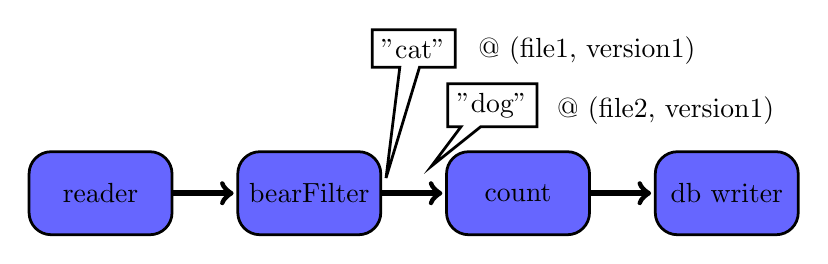
\begin{tikzpicture}[node distance = 0.8cm, auto]
\usetikzlibrary{shapes,arrows}
\usetikzlibrary{positioning}

\tikzstyle{operator} = [rectangle, draw, fill=blue!60, text width=4.5em, text centered, rounded corners = 8pt, minimum height=30pt, line width=1pt]
\tikzstyle{callout} = [draw, rectangle callout, callout relative pointer={#1}, line width=1pt]

    \node [operator] at (0, 0) (reader) {reader};
    \node [operator, right = of reader] (filter) {bearFilter};
    \node [operator, right = of filter] (count) {count};
    \node [operator, right = of count] (writer) {db writer};

    \draw [thick,->,shorten >=1pt, line width=2pt] (reader) -- (filter); 
    \draw [thick,->,shorten >=1pt, line width=2pt] (filter) -- (count) 
       node[callout={(-0.3,-40pt)}, midway,above = 45pt] {"cat"} node[midway,above= 45pt, shift={(2.2,-0.1)}] {@ (file1, version1)}
       node[callout={(-0.5,-0.5)}, midway,above= 15pt, shift={(1.0,0.3)}] {"dog"} node[midway,above= 15pt, shift={(3.2,0.2)}] {@ (file2, version1)};
     \draw [thick,->,shorten >=1pt, line width=2pt] (count) -- (writer); 
\end{tikzpicture}

  \end{center}
\end{frame}

\begin{frame}[fragile, noframenumbering]
  \frametitle{Example of a conventional Dataflow}
  \begin{center}
    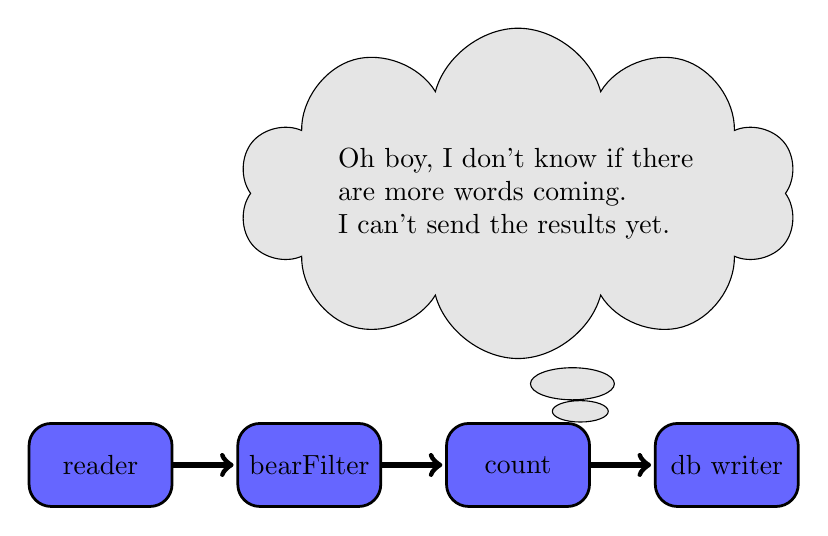
\begin{tikzpicture}[node distance = 0.8cm, auto]
\usetikzlibrary{shapes,arrows}
\usetikzlibrary{positioning}
\usetikzlibrary{calc,shapes.callouts,shapes.arrows}

\tikzstyle{operator} = [rectangle, draw, fill=blue!60, text width=4.5em, text centered, rounded corners = 8pt, minimum height=30pt, line width=1pt]
\tikzstyle{callout} = [draw, rectangle callout, callout relative pointer={#1}, line width=1pt]

    \node [operator] at (0, 0) (reader) {reader};
    \node [operator, right = of reader] (filter) {bearFilter};
    \node [operator, right = of filter] (count) {count}; 
    \node [operator, right = of count] (writer) {db writer};
    \node[draw,cloud callout,callout relative pointer={(0.2cm,-0.7cm)},  text width=13em, aspect=2.5,fill=black!10, above = of count] (hello) {Oh boy, I don't know if there are more words coming.\\I can't send the results yet.};

    \draw [thick,->,shorten >=1pt, line width=2pt] (reader) -- (filter); 
    \draw [thick,->,shorten >=1pt, line width=2pt] (filter) -- (count);
     \draw [thick,->,shorten >=1pt, line width=2pt] (count) -- (writer); 


\end{tikzpicture}

  \end{center}
\end{frame}

\begin{frame}[fragile, noframenumbering]
  \frametitle{Example of a conventional Dataflow}
  \begin{center}
    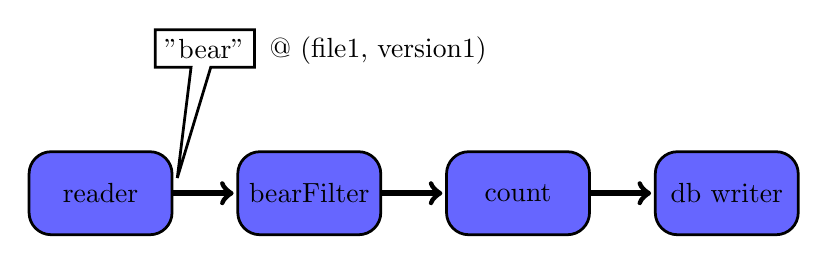
\begin{tikzpicture}[node distance = 0.8cm, auto]
\usetikzlibrary{shapes,arrows}
\usetikzlibrary{positioning}

\tikzstyle{operator} = [rectangle, draw, fill=blue!60, text width=4.5em, text centered, rounded corners = 8pt, minimum height=30pt, line width=1pt]
\tikzstyle{callout} = [draw, rectangle callout, callout relative pointer={#1}, line width=1pt]

    \node [operator] at (0, 0) (reader) {reader};
    \node [operator, right = of reader] (filter) {bearFilter};
    \node [operator, right = of filter] (count) {count};
    \node [operator, right = of count] (writer) {db writer};

    \draw [thick,->,shorten >=1pt, line width=2pt] (reader) -- (filter) 
       node[callout={(-0.3,-40pt)}, midway,above = 45pt] {"bear"} node[midway,above= 45pt, shift={(2.2,-0.1)}] {@ (file1, version1)};
    \draw [thick,->,shorten >=1pt, line width=2pt] (filter) -- (count); 
     \draw [thick,->,shorten >=1pt, line width=2pt] (count) -- (writer); 
\end{tikzpicture}

  \end{center}
\end{frame}

\begin{frame}[fragile, noframenumbering]
  \frametitle{Example of a conventional Dataflow}
  \begin{center}
    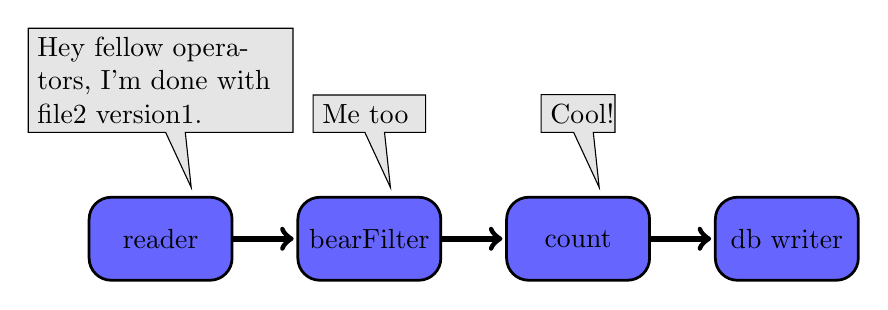
\begin{tikzpicture}[node distance = 0.8cm, auto]
\usetikzlibrary{shapes,arrows}
\usetikzlibrary{positioning}
\usetikzlibrary{calc,shapes.callouts,shapes.arrows}

\tikzstyle{operator} = [rectangle, draw, fill=blue!60, text width=4.5em, text centered, rounded corners = 8pt, minimum height=30pt, line width=1pt]
\tikzstyle{callout} = [draw, rectangle callout, callout relative pointer={#1}, line width=1pt]

    \node [operator] at (0, 0) (reader) {reader};
    \node [operator, right = of reader] (filter) {bearFilter};
    \node [operator, right = of filter] (count) {count}; 
    \node [operator, right = of count] (writer) {db writer};
    \node[draw, rectangle callout,callout relative pointer={(0.2cm,-0.7cm)},  text width=8.9em, aspect=2.5,fill=black!10, above = of reader] (hello) {Hey fellow operators, I'm done with file2 version1.};
    \node[draw, rectangle callout,callout relative pointer={(0.2cm,-0.7cm)},  text width=2em, aspect=2.5,fill=black!10, above = of count] (hello) {Cool!};
    \node[draw, rectangle callout,callout relative pointer={(0.2cm,-0.7cm)},  text width=3.4em, aspect=2.5,fill=black!10, above = of filter] (hello) {Me too};

    \draw [thick,->,shorten >=1pt, line width=2pt] (reader) -- (filter); 
    \draw [thick,->,shorten >=1pt, line width=2pt] (filter) -- (count);
     \draw [thick,->,shorten >=1pt, line width=2pt] (count) -- (writer); 


\end{tikzpicture}

  \end{center}
\end{frame}

\begin{frame}[fragile, noframenumbering]
  \frametitle{Example of a conventional Dataflow}
  \begin{center}
    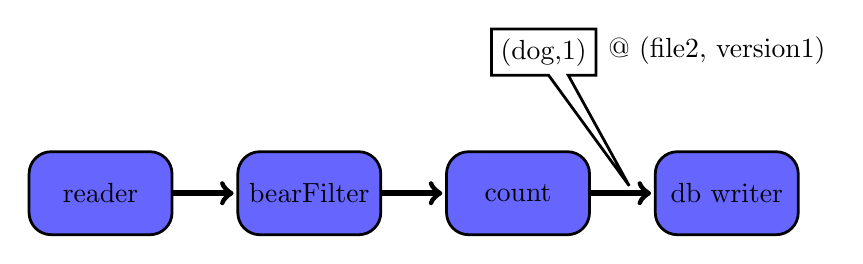
\begin{tikzpicture}[node distance = 0.8cm, auto]
\usetikzlibrary{shapes,arrows}
\usetikzlibrary{positioning}

\tikzstyle{operator} = [rectangle, draw, fill=blue!60, text width=4.5em, text centered, rounded corners = 8pt, minimum height=30pt, line width=1pt]
\tikzstyle{callout} = [draw, rectangle callout, callout relative pointer={#1}, line width=1pt]

    \node [operator] at (0, 0) (reader) {reader};
    \node [operator, right = of reader] (filter) {bearFilter};
    \node [operator, right = of filter] (count) {count};
    \node [operator, right = of count] (writer) {db writer};

    \draw [thick,->,shorten >=1pt, line width=2pt] (reader) -- (filter); 
    \draw [thick,->,shorten >=1pt, line width=2pt] (count) -- (writer) 
       node[callout={(0.9,-40pt)}, midway, shift={(-1,-0.1)}, above = 45pt] {(dog,1)} node[midway,above= 45pt, shift={(1.2,-0.1)}] {@ (file2, version1)};
     \draw [thick,->,shorten >=1pt, line width=2pt] (filter) -- (count); 
\end{tikzpicture}

  \end{center}
\end{frame}

\begin{frame}[fragile, noframenumbering]
  \frametitle{Example of a conventional Dataflow}
  \begin{center}
    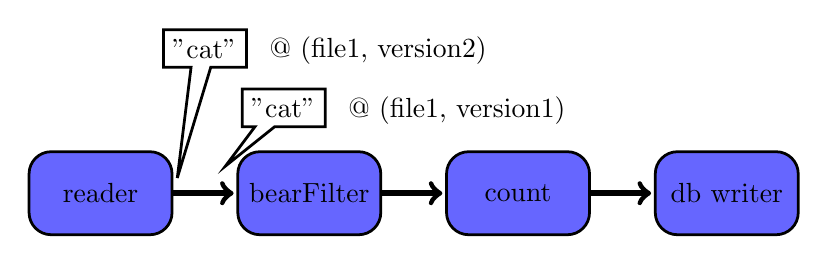
\begin{tikzpicture}[node distance = 0.8cm, auto]
\usetikzlibrary{shapes,arrows}
\usetikzlibrary{positioning}

\tikzstyle{operator} = [rectangle, draw, fill=blue!60, text width=4.5em, text centered, rounded corners = 8pt, minimum height=30pt, line width=1pt]
\tikzstyle{callout} = [draw, rectangle callout, callout relative pointer={#1}, line width=1pt]

    \node [operator] at (0, 0) (reader) {reader};
    \node [operator, right = of reader] (filter) {bearFilter};
    \node [operator, right = of filter] (count) {count};
    \node [operator, right = of count] (writer) {db writer};

    \draw [thick,->,shorten >=1pt, line width=2pt] (reader) -- (filter) 
       node[callout={(-0.3,-40pt)}, midway,above = 45pt] {"cat"} node[midway,above= 45pt, shift={(2.2,-0.1)}] {@ (file1, version2)}
       node[callout={(-0.5,-0.5)}, midway,above= 15pt, shift={(1.0,0.3)}] {"cat"} node[midway,above= 15pt, shift={(3.2,0.2)}] {@ (file1, version1)};
    \draw [thick,->,shorten >=1pt, line width=2pt] (filter) -- (count); 
     \draw [thick,->,shorten >=1pt, line width=2pt] (count) -- (writer); 
\end{tikzpicture}

  \end{center}
\end{frame}

\begin{frame}[fragile, noframenumbering]
  \frametitle{Example of a conventional Dataflow}
  \begin{center}
    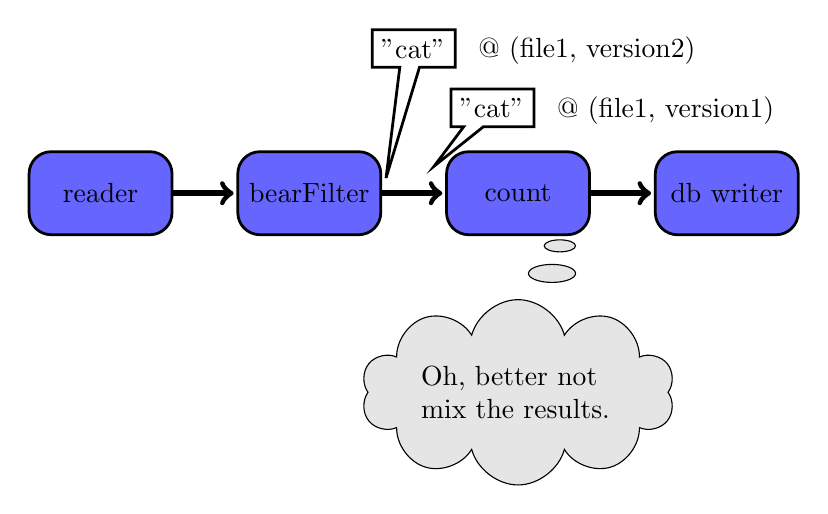
\begin{tikzpicture}[node distance = 0.8cm, auto]
\usetikzlibrary{shapes,arrows}
\usetikzlibrary{positioning}

\tikzstyle{operator} = [rectangle, draw, fill=blue!60, text width=4.5em, text centered, rounded corners = 8pt, minimum height=30pt, line width=1pt]
\tikzstyle{callout} = [draw, rectangle callout, callout relative pointer={#1}, line width=1pt]

    \node [operator] at (0, 0) (reader) {reader};
    \node [operator, right = of reader] (filter) {bearFilter};
    \node [operator, right = of filter] (count) {count};
    \node [operator, right = of count] (writer) {db writer};
    \node[draw,cloud callout,callout relative pointer={(0.2cm,0.7cm)},  text width=7em, aspect=2.5,fill=black!10, below = of count] (hello) {Oh, better not mix the results.};

    \draw [thick,->,shorten >=1pt, line width=2pt] (filter) -- (count) 
       node[callout={(-0.3,-40pt)}, midway,above = 45pt] {"cat"} node[midway,above= 45pt, shift={(2.2,-0.1)}] {@ (file1, version2)}
       node[callout={(-0.5,-0.5)}, midway,above= 15pt, shift={(1.0,0.3)}] {"cat"} node[midway,above= 15pt, shift={(3.2,0.2)}] {@ (file1, version1)};
    \draw [thick,->,shorten >=1pt, line width=2pt] (reader) -- (filter); 
     \draw [thick,->,shorten >=1pt, line width=2pt] (count) -- (writer); 
\end{tikzpicture}

  \end{center}
\end{frame}

\begin{frame}[fragile, noframenumbering]
  \frametitle{Example of a conventional Dataflow}
  \begin{center}
    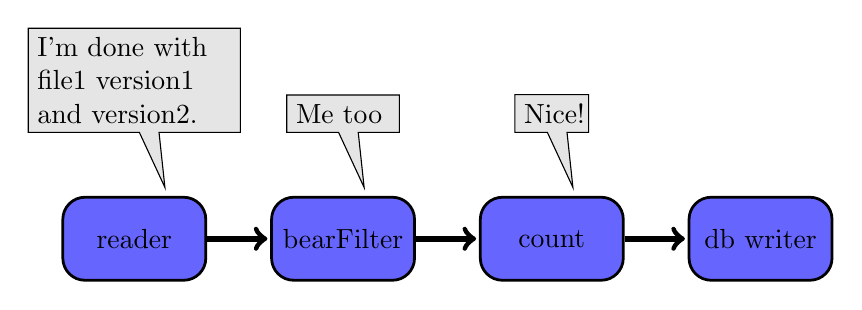
\begin{tikzpicture}[node distance = 0.8cm, auto]
\usetikzlibrary{shapes,arrows}
\usetikzlibrary{positioning}
\usetikzlibrary{calc,shapes.callouts,shapes.arrows}

\tikzstyle{operator} = [rectangle, draw, fill=blue!60, text width=4.5em, text centered, rounded corners = 8pt, minimum height=30pt, line width=1pt]
\tikzstyle{callout} = [draw, rectangle callout, callout relative pointer={#1}, line width=1pt]

    \node [operator] at (0, 0) (reader) {reader};
    \node [operator, right = of reader] (filter) {bearFilter};
    \node [operator, right = of filter] (count) {count}; 
    \node [operator, right = of count] (writer) {db writer};
    \node[draw, rectangle callout,callout relative pointer={(0.2cm,-0.7cm)},  text width=7em, aspect=2.5,fill=black!10, above = of reader] (hello) {I'm done with file1 version1 and version2.};
    \node[draw, rectangle callout,callout relative pointer={(0.2cm,-0.7cm)},  text width=2em, aspect=2.5,fill=black!10, above = of count] (hello) {Nice!};
   \node[draw, rectangle callout,callout relative pointer={(0.2cm,-0.7cm)},  text width=3.4em, aspect=2.5,fill=black!10, above = of filter] (hello) {Me too};

    \draw [thick,->,shorten >=1pt, line width=2pt] (reader) -- (filter); 
    \draw [thick,->,shorten >=1pt, line width=2pt] (filter) -- (count);
     \draw [thick,->,shorten >=1pt, line width=2pt] (count) -- (writer); 


\end{tikzpicture}

  \end{center}
\end{frame}

\begin{frame}[fragile]
  \frametitle{Example of a conventional Dataflow with a cycle}
  \begin{center}
    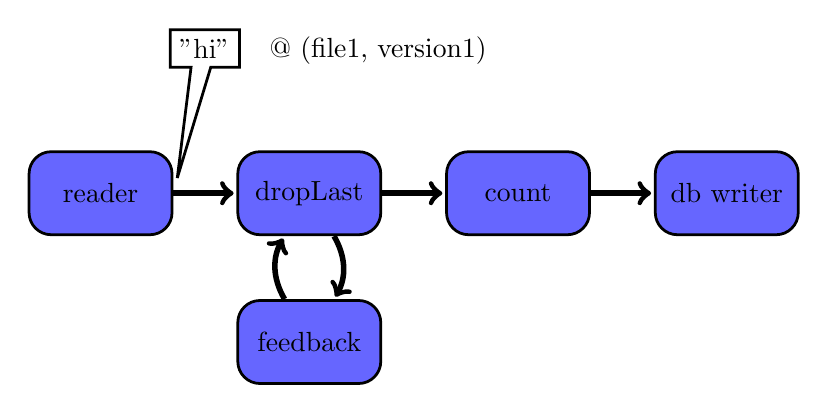
\begin{tikzpicture}[node distance = 0.8cm, auto]
\usetikzlibrary{shapes,arrows}
\usetikzlibrary{positioning}

\tikzstyle{operator} = [rectangle, draw, fill=blue!60, text width=4.5em, text centered, rounded corners = 8pt, minimum height=30pt, line width=1pt]
\tikzstyle{callout} = [draw, rectangle callout, callout relative pointer={#1}, line width=1pt]

    \node [operator] at (0, 0) (reader) {reader};
    \node [operator, right = of reader] (filter) {dropLast};
    \node [operator, right = of filter] (count) {count};
    \node [operator, below = of filter] (feedback) {feedback};
    \node [operator, right = of count] (writer) {db writer};

    \draw [thick,->,shorten >=1pt, line width=2pt] (reader) -- (filter) 
       node[callout={(-0.3,-40pt)}, midway,above = 45pt] {"hi"} node[midway,above= 45pt, shift={(2.2,-0.1)}] {@ (file1, version1)};
    \draw [thick,->,shorten >=1pt, line width=2pt] (filter) -- (count); 
     \draw [thick,->,shorten >=1pt, line width=2pt] (count) -- (writer); 
    \draw [thick,->,shorten >=1pt, line width=2pt] (filter) edge  [bend left]  (feedback); 
     \draw [thick,->,shorten >=1pt, line width=2pt] (feedback) edge  [bend left]  (filter); 
\end{tikzpicture}

  \end{center}
\end{frame}

\begin{frame}[fragile, noframenumbering]
  \frametitle{Example of a conventional Dataflow with a cycle}
  \begin{center}
    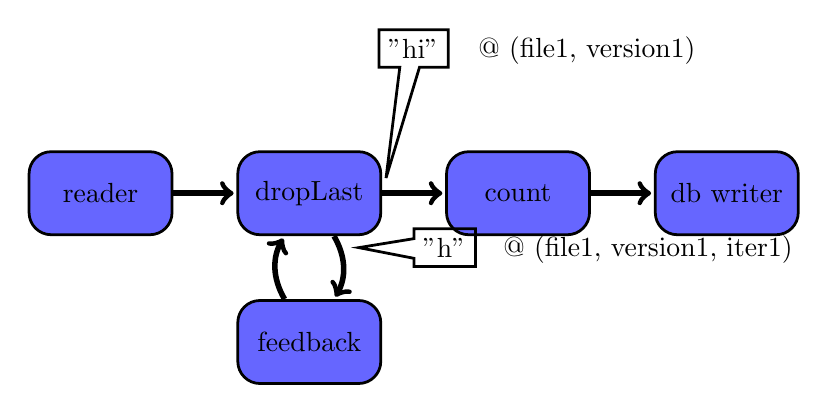
\begin{tikzpicture}[node distance = 0.8cm, auto]
\usetikzlibrary{shapes,arrows}
\usetikzlibrary{positioning}

\tikzstyle{operator} = [rectangle, draw, fill=blue!60, text width=4.5em, text centered, rounded corners = 8pt, minimum height=30pt, line width=1pt]
\tikzstyle{callout} = [draw, rectangle callout, callout relative pointer={#1}, line width=1pt]

    \node [operator] at (0, 0) (reader) {reader};
    \node [operator, right = of reader] (filter) {dropLast};
    \node [operator, right = of filter] (count) {count};
    \node [operator, below = of filter] (feedback) {feedback};
    \node [operator, right = of count] (writer) {db writer};

    \draw [thick,->,shorten >=1pt, line width=2pt] (reader) -- (filter) ;
    \draw [thick,->,shorten >=1pt, line width=2pt] (filter) -- (count)
       node[callout={(-0.3,-40pt)}, midway,above = 45pt] {"hi"} node[midway,above= 45pt, shift={(2.2,-0.1)}] {@ (file1, version1)}; 
     \draw [thick,->,shorten >=1pt, line width=2pt] (count) -- (writer); 
    \draw [thick,->,shorten >=1pt, line width=2pt] (filter) to  [bend left]  (feedback)  
      node[callout={(-0.7,0pt)}, above right  = 20pt , shift={(0.5,-0.1)}] {"h"} node[ above right  = 20pt , shift={(1.5,-0.2)}] {@ (file1, version1, iter1)}; 
     \draw [thick,->,shorten >=1pt, line width=2pt] (feedback) edge  [bend left]  (filter); 
\end{tikzpicture}

  \end{center}
\end{frame}

\begin{frame}[fragile, noframenumbering]
  \frametitle{Example of a conventional Dataflow with a cycle}
  \begin{center}
    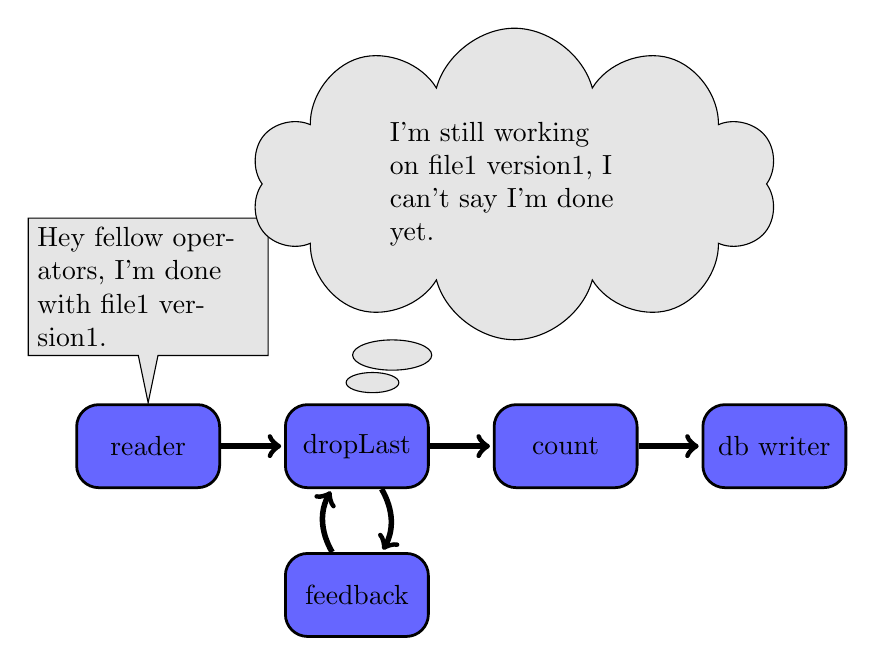
\begin{tikzpicture}[node distance = 0.8cm, auto]
\usetikzlibrary{shapes,arrows}
\usetikzlibrary{positioning}

\tikzstyle{operator} = [rectangle, draw, fill=blue!60, text width=4.5em, text centered, rounded corners = 8pt, minimum height=30pt, line width=1pt]
\tikzstyle{callout} = [draw, rectangle callout, callout relative pointer={#1}, line width=1pt]

    \node [operator] at (0, 0) (reader) {reader};
    \node [operator, right = of reader] (filter) {dropLast};
    \node [operator, right = of filter] (count) {count};
    \node [operator, below = of filter] (feedback) {feedback};
   \node[draw, rectangle callout,callout relative pointer={(0cm,-0.6cm)}, shift={(0,-0.2)},  text width=8em, aspect=2.5,fill=black!10, above = of reader] (hello) {Hey fellow operators, I'm done with file1 version1.};
    \node [operator, right = of count] (writer) {db writer};
        \node[draw,cloud callout,callout relative pointer={(-0.5cm,-0.7cm)},  text width=9em, aspect=2.5,fill=black!10, above = of filter, shift={(2,0)}] (hello) {I'm still working on file1 version1, I can't say I'm done yet.};


    \draw [thick,->,shorten >=1pt, line width=2pt] (reader) -- (filter) ;
    \draw [thick,->,shorten >=1pt, line width=2pt] (filter) -- (count); 
     \draw [thick,->,shorten >=1pt, line width=2pt] (count) -- (writer); 
    \draw [thick,->,shorten >=1pt, line width=2pt] (filter) to  [bend left]  (feedback); 
     \draw [thick,->,shorten >=1pt, line width=2pt] (feedback) edge  [bend left]  (filter); 
\end{tikzpicture}

  \end{center}
\end{frame}

\begin{frame}[fragile, noframenumbering]
  \frametitle{Example of a conventional Dataflow with a cycle}
  \begin{center}
    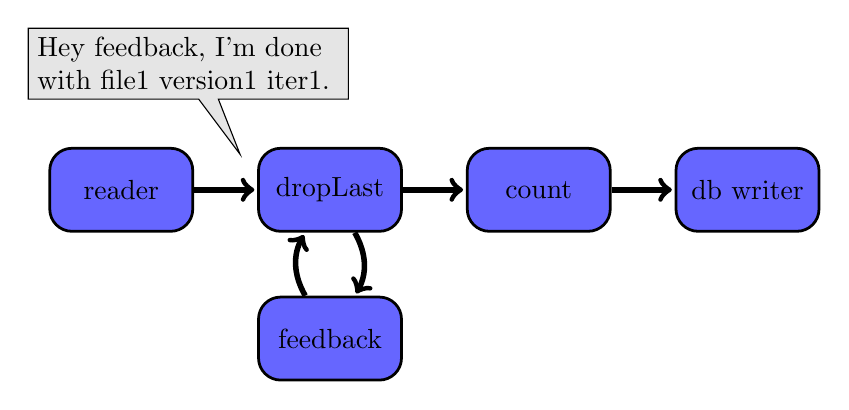
\begin{tikzpicture}[node distance = 0.8cm, auto]
\usetikzlibrary{shapes,arrows}
\usetikzlibrary{positioning}

\tikzstyle{operator} = [rectangle, draw, fill=blue!60, text width=4.5em, text centered, rounded corners = 8pt, minimum height=30pt, line width=1pt]
\tikzstyle{callout} = [draw, rectangle callout, callout relative pointer={#1}, line width=1pt]

    \node [operator] at (0, 0) (reader) {reader};
    \node [operator, right = of reader] (filter) {dropLast};
    \node [operator, right = of filter] (count) {count};
    \node [operator, below = of filter] (feedback) {feedback};
   \node[draw, rectangle callout,callout relative pointer={(0.4cm,-0.7cm)}, shift={(-1.8,-0.2)},  text width=10.9em, aspect=2.5,fill=black!10, above = of filter] (hello) {Hey feedback, I'm done with file1 version1 iter1.};
    \node [operator, right = of count] (writer) {db writer};


    \draw [thick,->,shorten >=1pt, line width=2pt] (reader) -- (filter) ;
    \draw [thick,->,shorten >=1pt, line width=2pt] (filter) -- (count); 
     \draw [thick,->,shorten >=1pt, line width=2pt] (count) -- (writer); 
    \draw [thick,->,shorten >=1pt, line width=2pt] (filter) to  [bend left]  (feedback); 
     \draw [thick,->,shorten >=1pt, line width=2pt] (feedback) edge  [bend left]  (filter); 
\end{tikzpicture}

  \end{center}
\end{frame}

\begin{frame}[fragile, noframenumbering]
  \frametitle{Example of a conventional Dataflow with a cycle}
  \begin{center}
    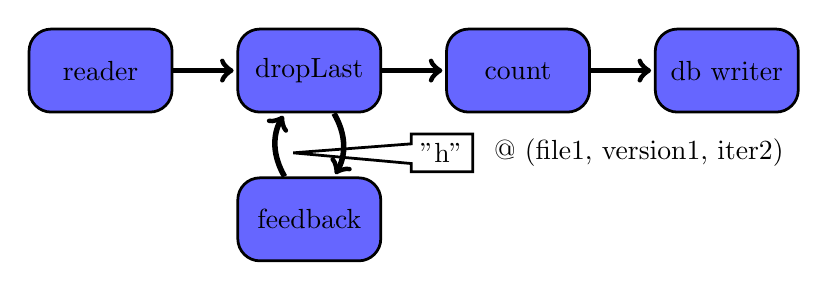
\begin{tikzpicture}[node distance = 0.8cm, auto]
\usetikzlibrary{shapes,arrows}
\usetikzlibrary{positioning}

\tikzstyle{operator} = [rectangle, draw, fill=blue!60, text width=4.5em, text centered, rounded corners = 8pt, minimum height=30pt, line width=1pt]
\tikzstyle{callout} = [draw, rectangle callout, callout relative pointer={#1}, line width=1pt]

    \node [operator] at (0, 0) (reader) {reader};
    \node [operator, right = of reader] (filter) {dropLast};
    \node [operator, right = of filter] (count) {count};
    \node [operator, below = of filter] (feedback) {feedback};
    \node [operator, right = of count] (writer) {db writer};


    \draw [thick,->,shorten >=1pt, line width=2pt] (reader) -- (filter) ;
    \draw [thick,->,shorten >=1pt, line width=2pt] (filter) -- (count); 
     \draw [thick,->,shorten >=1pt, line width=2pt] (count) -- (writer); 
    \draw [thick,->,shorten >=1pt, line width=2pt] (filter) to  [bend left]  (feedback); 
     \draw [thick,->,shorten >=1pt, line width=2pt] (feedback) to  [bend left]  (filter)
node[callout={(-1.5,0pt)}, shift={(2.0,-0.5)}] {"h"} node[shift={(4.5,-0.5)}] {@ (file1, version1, iter2)}; 
\end{tikzpicture}

  \end{center}
\end{frame}

\begin{frame}[fragile, noframenumbering]
  \frametitle{Example of a conventional Dataflow with a cycle}
  \begin{center}
    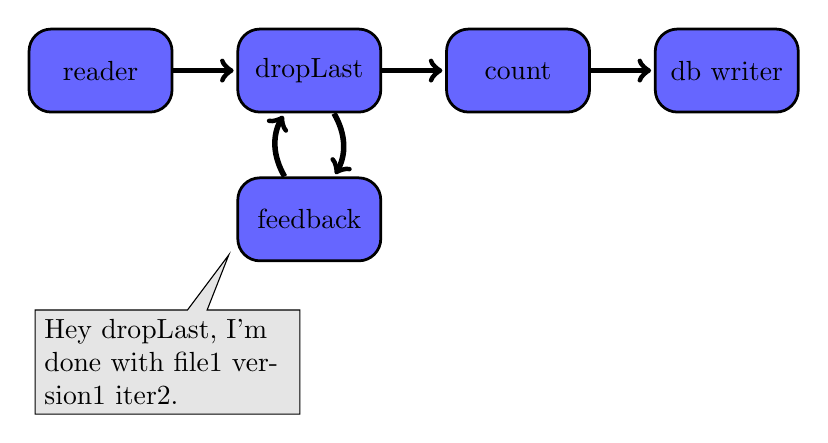
\begin{tikzpicture}[node distance = 0.8cm, auto]
\usetikzlibrary{shapes,arrows}
\usetikzlibrary{positioning}

\tikzstyle{operator} = [rectangle, draw, fill=blue!60, text width=4.5em, text centered, rounded corners = 8pt, minimum height=30pt, line width=1pt]
\tikzstyle{callout} = [draw, rectangle callout, callout relative pointer={#1}, line width=1pt]

    \node [operator] at (0, 0) (reader) {reader};
    \node [operator, right = of reader] (filter) {dropLast};
    \node [operator, right = of filter] (count) {count};
    \node [operator, below = of filter] (feedback) {feedback};
    \node [operator, right = of count] (writer) {db writer};
   \node[draw, rectangle callout,callout relative pointer={(0.4cm,0.7cm)}, shift={(-1.8,0.2)},  text width=8.9em, aspect=2.5,fill=black!10, below = of feedback] (hello) {Hey dropLast, I'm done with file1 version1 iter2.};


    \draw [thick,->,shorten >=1pt, line width=2pt] (reader) -- (filter) ;
    \draw [thick,->,shorten >=1pt, line width=2pt] (filter) -- (count); 
     \draw [thick,->,shorten >=1pt, line width=2pt] (count) -- (writer); 
    \draw [thick,->,shorten >=1pt, line width=2pt] (filter) to  [bend left]  (feedback); 
     \draw [thick,->,shorten >=1pt, line width=2pt] (feedback) to  [bend left]  (filter); 
\end{tikzpicture}

  \end{center}
\end{frame}

\begin{frame}[fragile, noframenumbering]
  \frametitle{Example of a conventional Dataflow with a cycle}
  \begin{center}
    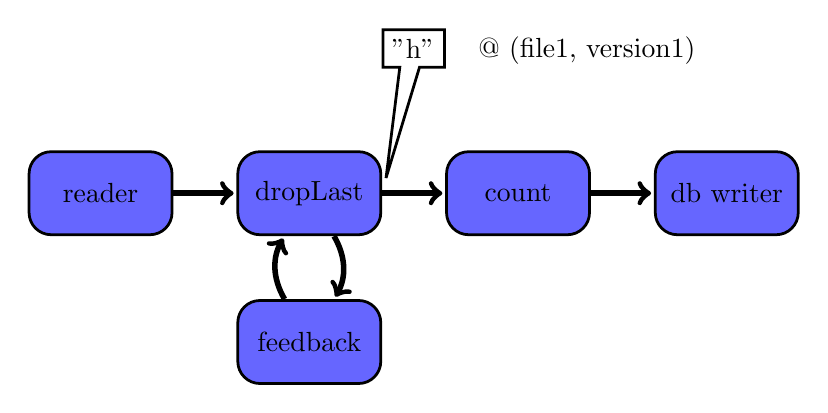
\begin{tikzpicture}[node distance = 0.8cm, auto]
\usetikzlibrary{shapes,arrows}
\usetikzlibrary{positioning}

\tikzstyle{operator} = [rectangle, draw, fill=blue!60, text width=4.5em, text centered, rounded corners = 8pt, minimum height=30pt, line width=1pt]
\tikzstyle{callout} = [draw, rectangle callout, callout relative pointer={#1}, line width=1pt]

    \node [operator] at (0, 0) (reader) {reader};
    \node [operator, right = of reader] (filter) {dropLast};
    \node [operator, right = of filter] (count) {count};
    \node [operator, below = of filter] (feedback) {feedback};
    \node [operator, right = of count] (writer) {db writer};

    \draw [thick,->,shorten >=1pt, line width=2pt] (reader) -- (filter) ;
    \draw [thick,->,shorten >=1pt, line width=2pt] (filter) -- (count)
       node[callout={(-0.3,-40pt)}, midway,above = 45pt] {"h"} node[midway,above= 45pt, shift={(2.2,-0.1)}] {@ (file1, version1)}; 
     \draw [thick,->,shorten >=1pt, line width=2pt] (count) -- (writer); 
    \draw [thick,->,shorten >=1pt, line width=2pt] (filter) to  [bend left]  (feedback) ; 
     \draw [thick,->,shorten >=1pt, line width=2pt] (feedback) edge  [bend left]  (filter); 
\end{tikzpicture}

  \end{center}
\end{frame}

\begin{frame}[fragile, noframenumbering]
  \frametitle{Example of a conventional Dataflow with a cycle}
  \begin{center}
    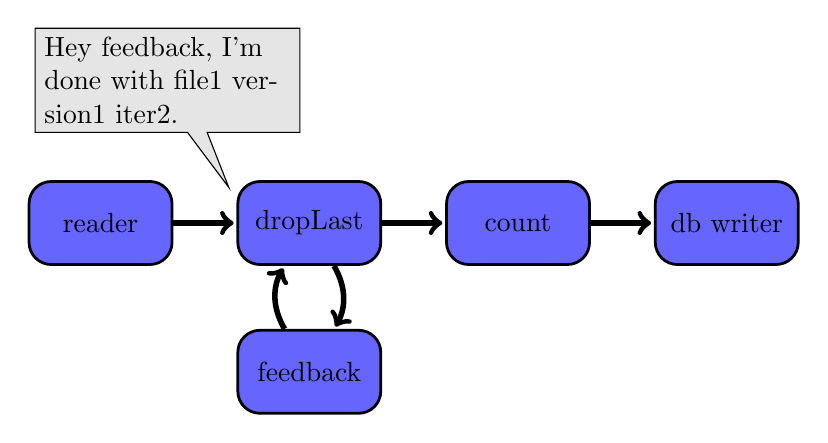
\begin{tikzpicture}[node distance = 0.8cm, auto]
\usetikzlibrary{shapes,arrows}
\usetikzlibrary{positioning}

\tikzstyle{operator} = [rectangle, draw, fill=blue!60, text width=4.5em, text centered, rounded corners = 8pt, minimum height=30pt, line width=1pt]
\tikzstyle{callout} = [draw, rectangle callout, callout relative pointer={#1}, line width=1pt]

    \node [operator] at (0, 0) (reader) {reader};
    \node [operator, right = of reader] (filter) {dropLast};
    \node [operator, right = of filter] (count) {count};
    \node [operator, below = of filter] (feedback) {feedback};
   \node[draw, rectangle callout,callout relative pointer={(0.4cm,-0.7cm)}, shift={(-1.8,-0.2)},  text width=8.9em, aspect=2.5,fill=black!10, above = of filter] (hello) {Hey feedback, I'm done with file1 version1 iter2.};
    \node [operator, right = of count] (writer) {db writer};


    \draw [thick,->,shorten >=1pt, line width=2pt] (reader) -- (filter) ;
    \draw [thick,->,shorten >=1pt, line width=2pt] (filter) -- (count); 
     \draw [thick,->,shorten >=1pt, line width=2pt] (count) -- (writer); 
    \draw [thick,->,shorten >=1pt, line width=2pt] (filter) to  [bend left]  (feedback); 
     \draw [thick,->,shorten >=1pt, line width=2pt] (feedback) edge  [bend left]  (filter); 
\end{tikzpicture}

  \end{center}
\end{frame}

\begin{frame}[fragile, noframenumbering]
  \frametitle{Example of a conventional Dataflow with a cycle}
  \begin{center}
    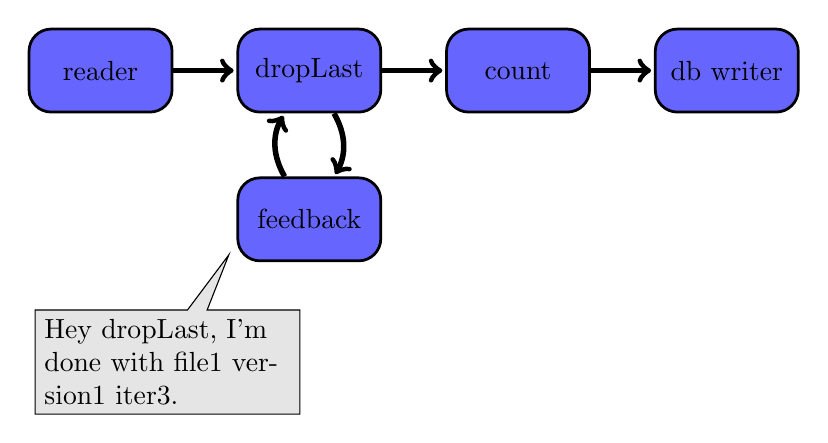
\begin{tikzpicture}[node distance = 0.8cm, auto]
\usetikzlibrary{shapes,arrows}
\usetikzlibrary{positioning}

\tikzstyle{operator} = [rectangle, draw, fill=blue!60, text width=4.5em, text centered, rounded corners = 8pt, minimum height=30pt, line width=1pt]
\tikzstyle{callout} = [draw, rectangle callout, callout relative pointer={#1}, line width=1pt]

    \node [operator] at (0, 0) (reader) {reader};
    \node [operator, right = of reader] (filter) {dropLast};
    \node [operator, right = of filter] (count) {count};
    \node [operator, below = of filter] (feedback) {feedback};
    \node [operator, right = of count] (writer) {db writer};
   \node[draw, rectangle callout,callout relative pointer={(0.4cm,0.7cm)}, shift={(-1.8,0.2)},  text width=8.9em, aspect=2.5,fill=black!10, below = of feedback] (hello) {Hey dropLast, I'm done with file1 version1 iter3.};


    \draw [thick,->,shorten >=1pt, line width=2pt] (reader) -- (filter) ;
    \draw [thick,->,shorten >=1pt, line width=2pt] (filter) -- (count); 
     \draw [thick,->,shorten >=1pt, line width=2pt] (count) -- (writer); 
    \draw [thick,->,shorten >=1pt, line width=2pt] (filter) to  [bend left]  (feedback); 
     \draw [thick,->,shorten >=1pt, line width=2pt] (feedback) to  [bend left]  (filter); 
\end{tikzpicture}

  \end{center}
\end{frame}

\begin{frame}
  \frametitle{Timely Dataflow}
  \begin{figure}
    \shadowbox{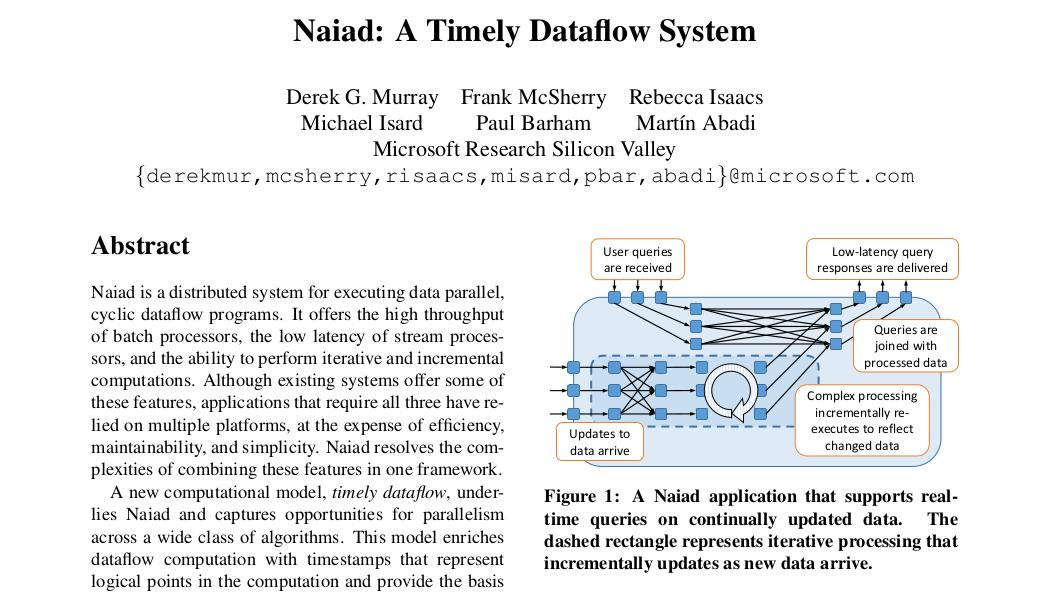
\includegraphics[width=0.5\textwidth]{naiad.jpg}}
  \end{figure}
  \pause
  \begin{itemize}
    \item Iterative computation (cycles)
          \pause
    \item Reports on the presence of data instead of the absence
          \pause
    \item Two implementations: C\# (Naiad) and Rust
  \end{itemize}
\end{frame}

\section{Progress Tracking}

\begin{frame}
  \frametitle{Progress Tracking Protocolllll}
  \begin{itemize}
    \item Two core components: Local Propagation and Distributed Exchange
          \begin{itemize}
            \item Local: localy compute the frontiers
                  \begin{itemize}
                    \item \textit{A frontier is a lower bound on the timestamps that may appear at the operator instance inputs}
                  \end{itemize}
            \item Exchange the timestamps between workers
          \end{itemize}
          \pause
    \item For every worker and for every location of the graph a conservative approximation of which timestamps may still arrive (a.ka. frontier)
  \end{itemize}
\end{frame}

\begin{frame}
  \frametitle{Local Propagation Example}
  \begin{center}
    \usetikzlibrary{shapes,arrows}
\usetikzlibrary{positioning}
\usetikzlibrary{calc,shapes.callouts,shapes.arrows}

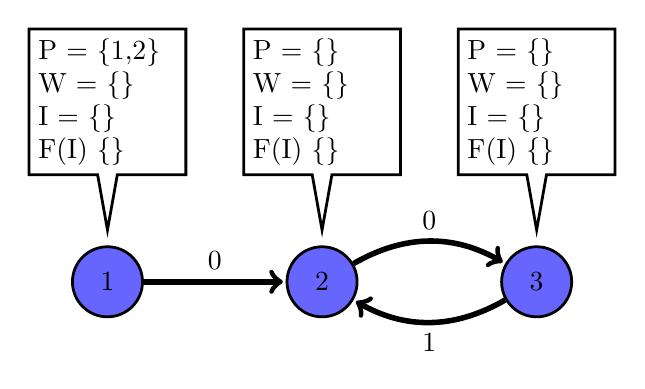
\begin{tikzpicture}[node distance = 1.8cm, auto]


\tikzstyle{operator} = [circle, draw, fill=blue!60, text width=1.5em, text centered, line width=1pt]

    \node [operator] at (0, 0) (1) {1};
    \node[draw, rectangle callout, above = of 1, line width=1pt, text width=5em, callout relative pointer={(0cm,-0.7cm)},above= 25pt] 
   { 
     P = \{1,2\}\\
     W = \{\}\\
     I = \{\}\\
     F(I) \{\}
    };

    \node [operator, right = of 1] (2) {2};
     \node[draw, rectangle callout, above = of 2, line width=1pt, text width=5em, callout relative pointer={(0cm,-0.7cm)},above= 25pt] 
   { 
     P = \{\}\\
     W = \{\}\\
     I = \{\}\\
     F(I) \{\}
    };

    \node [operator, right = of 2] (3) {3}; 
     \node[draw, rectangle callout, above = of 3, line width=1pt, text width=5em, callout relative pointer={(0cm,-0.7cm)},above= 25pt] 
   { 
     P = \{\}\\
     W = \{\}\\
     I = \{\}\\
     F(I) \{\}
    };


    \draw [thick,->,shorten >=1pt, line width=2pt] (1) edge node {0} (2); 
    \draw [thick,->,shorten >=1pt, line width=2pt] (2) edge  [bend left]  node {0} (3);
     \draw [thick,->,shorten >=1pt, line width=2pt] (3) edge  [bend left]  node {1} (2); 


\end{tikzpicture}

  \end{center}
\end{frame}

\begin{frame}[fragile, noframenumbering]
  \frametitle{Local Propagation Example}
  \begin{center}
    \usetikzlibrary{shapes,arrows}
\usetikzlibrary{positioning}
\usetikzlibrary{calc,shapes.callouts,shapes.arrows}

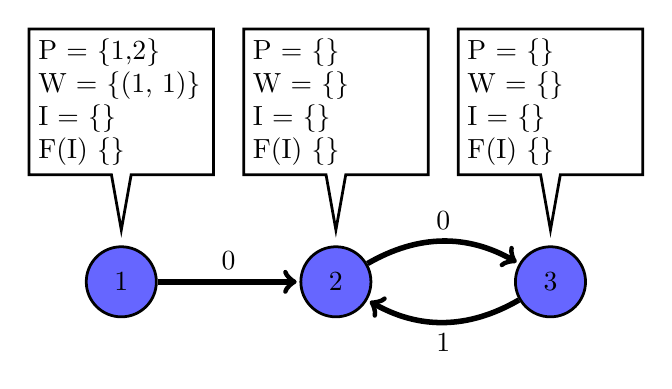
\begin{tikzpicture}[node distance = 1.8cm, auto]


\tikzstyle{operator} = [circle, draw, fill=blue!60, text width=1.5em, text centered, line width=1pt]

    \node [operator] at (0, 0) (1) {1};
    \node[draw, rectangle callout, above = of 1, line width=1pt, text width=6em, callout relative pointer={(0cm,-0.7cm)},above= 25pt] 
   { 
     P = \{1,2\}\\
     W = \{(1, 1)\}\\
     I = \{\}\\
     F(I) \{\}
    };

    \node [operator, right = of 1] (2) {2};
     \node[draw, rectangle callout, above = of 2, line width=1pt, text width=6em, callout relative pointer={(0cm,-0.7cm)},above= 25pt] 
   { 
     P = \{\}\\
     W = \{\}\\
     I = \{\}\\
     F(I) \{\}
    };

    \node [operator, right = of 2] (3) {3}; 
     \node[draw, rectangle callout, above = of 3, line width=1pt, text width=6em, callout relative pointer={(0cm,-0.7cm)},above= 25pt] 
   { 
     P = \{\}\\
     W = \{\}\\
     I = \{\}\\
     F(I) \{\}
    };


    \draw [thick,->,shorten >=1pt, line width=2pt] (1) edge node {0} (2); 
    \draw [thick,->,shorten >=1pt, line width=2pt] (2) edge  [bend left]  node {0} (3);
     \draw [thick,->,shorten >=1pt, line width=2pt] (3) edge  [bend left]  node {1} (2); 


\end{tikzpicture}

  \end{center}
\end{frame}

\begin{frame}[fragile, noframenumbering]
  \frametitle{Local Propagation Example}
  \begin{center}
    \usetikzlibrary{shapes,arrows}
\usetikzlibrary{positioning}
\usetikzlibrary{calc,shapes.callouts,shapes.arrows}

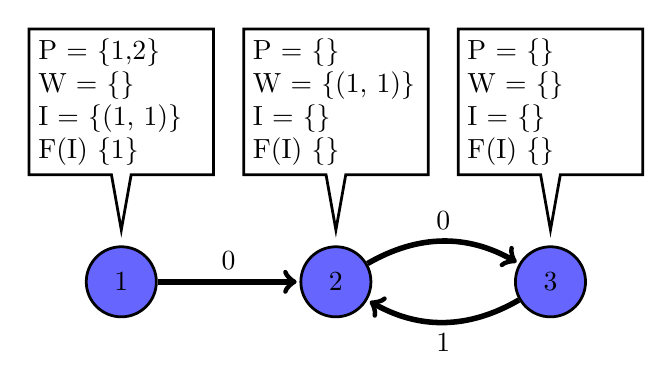
\begin{tikzpicture}[node distance = 1.8cm, auto]


\tikzstyle{operator} = [circle, draw, fill=blue!60, text width=1.5em, text centered, line width=1pt]

    \node [operator] at (0, 0) (1) {1};
    \node[draw, rectangle callout, above = of 1, line width=1pt, text width=6em, callout relative pointer={(0cm,-0.7cm)},above= 25pt] 
   { 
     P = \{1,2\}\\
     W = \{\}\\
     I = \{(1, 1)\}\\
     F(I) \{1\}
    };

    \node [operator, right = of 1] (2) {2};
     \node[draw, rectangle callout, above = of 2, line width=1pt, text width=6em, callout relative pointer={(0cm,-0.7cm)},above= 25pt] 
   { 
     P = \{\}\\
     W = \{(1, 1)\}\\
     I = \{\}\\
     F(I) \{\}
    };

    \node [operator, right = of 2] (3) {3}; 
     \node[draw, rectangle callout, above = of 3, line width=1pt, text width=6em, callout relative pointer={(0cm,-0.7cm)},above= 25pt] 
   { 
     P = \{\}\\
     W = \{\}\\
     I = \{\}\\
     F(I) \{\}
    };


    \draw [thick,->,shorten >=1pt, line width=2pt] (1) edge node {0} (2); 
    \draw [thick,->,shorten >=1pt, line width=2pt] (2) edge  [bend left]  node {0} (3);
     \draw [thick,->,shorten >=1pt, line width=2pt] (3) edge  [bend left]  node {1} (2); 


\end{tikzpicture}

  \end{center}
\end{frame}

\begin{frame}[fragile, noframenumbering]
  \frametitle{Local Propagation Example}
  \begin{center}
    \usetikzlibrary{shapes,arrows}
\usetikzlibrary{positioning}
\usetikzlibrary{calc,shapes.callouts,shapes.arrows}

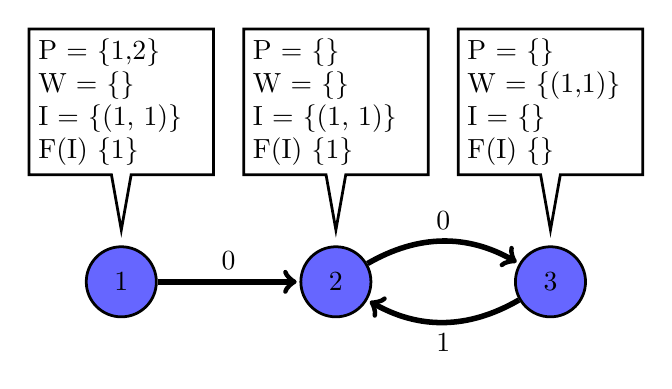
\begin{tikzpicture}[node distance = 1.8cm, auto]


\tikzstyle{operator} = [circle, draw, fill=blue!60, text width=1.5em, text centered, line width=1pt]

    \node [operator] at (0, 0) (1) {1};
    \node[draw, rectangle callout, above = of 1, line width=1pt, text width=6em, callout relative pointer={(0cm,-0.7cm)},above= 25pt] 
   { 
     P = \{1,2\}\\
     W = \{\}\\
     I = \{(1, 1)\}\\
     F(I) \{1\}
    };

    \node [operator, right = of 1] (2) {2};
     \node[draw, rectangle callout, above = of 2, line width=1pt, text width=6em, callout relative pointer={(0cm,-0.7cm)},above= 25pt] 
   { 
     P = \{\}\\
     W = \{\}\\
     I = \{(1, 1)\}\\
     F(I) \{1\}
    };

    \node [operator, right = of 2] (3) {3}; 
     \node[draw, rectangle callout, above = of 3, line width=1pt, text width=6em, callout relative pointer={(0cm,-0.7cm)},above= 25pt] 
   { 
     P = \{\}\\
     W = \{(1,1)\}\\
     I = \{\}\\
     F(I) \{\}
    };


    \draw [thick,->,shorten >=1pt, line width=2pt] (1) edge node {0} (2); 
    \draw [thick,->,shorten >=1pt, line width=2pt] (2) edge  [bend left]  node {0} (3);
     \draw [thick,->,shorten >=1pt, line width=2pt] (3) edge  [bend left]  node {1} (2); 


\end{tikzpicture}

  \end{center}
\end{frame}

\begin{frame}[fragile, noframenumbering]
  \frametitle{Local Propagation Example}
  \begin{center}
    \usetikzlibrary{shapes,arrows}
\usetikzlibrary{positioning}
\usetikzlibrary{calc,shapes.callouts,shapes.arrows}

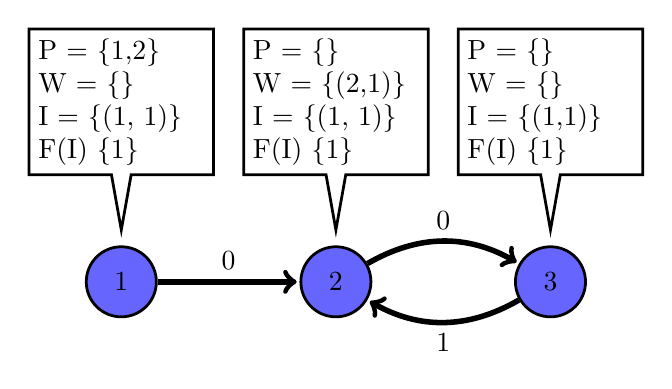
\begin{tikzpicture}[node distance = 1.8cm, auto]


\tikzstyle{operator} = [circle, draw, fill=blue!60, text width=1.5em, text centered, line width=1pt]

    \node [operator] at (0, 0) (1) {1};
    \node[draw, rectangle callout, above = of 1, line width=1pt, text width=6em, callout relative pointer={(0cm,-0.7cm)},above= 25pt] 
   { 
     P = \{1,2\}\\
     W = \{\}\\
     I = \{(1, 1)\}\\
     F(I) \{1\}
    };

    \node [operator, right = of 1] (2) {2};
     \node[draw, rectangle callout, above = of 2, line width=1pt, text width=6em, callout relative pointer={(0cm,-0.7cm)},above= 25pt] 
   { 
     P = \{\}\\
     W = \{(2,1)\}\\
     I = \{(1, 1)\}\\
     F(I) \{1\}
    };

    \node [operator, right = of 2] (3) {3}; 
     \node[draw, rectangle callout, above = of 3, line width=1pt, text width=6em, callout relative pointer={(0cm,-0.7cm)},above= 25pt] 
   { 
     P = \{\}\\
     W = \{\}\\
     I = \{(1,1)\}\\
     F(I) \{1\}
    };


    \draw [thick,->,shorten >=1pt, line width=2pt] (1) edge node {0} (2); 
    \draw [thick,->,shorten >=1pt, line width=2pt] (2) edge  [bend left]  node {0} (3);
     \draw [thick,->,shorten >=1pt, line width=2pt] (3) edge  [bend left]  node {1} (2); 


\end{tikzpicture}

  \end{center}
\end{frame}

\begin{frame}[fragile, noframenumbering]
  \frametitle{Local Propagation Example}
  \begin{center}
    \usetikzlibrary{shapes,arrows}
\usetikzlibrary{positioning}
\usetikzlibrary{calc,shapes.callouts,shapes.arrows}

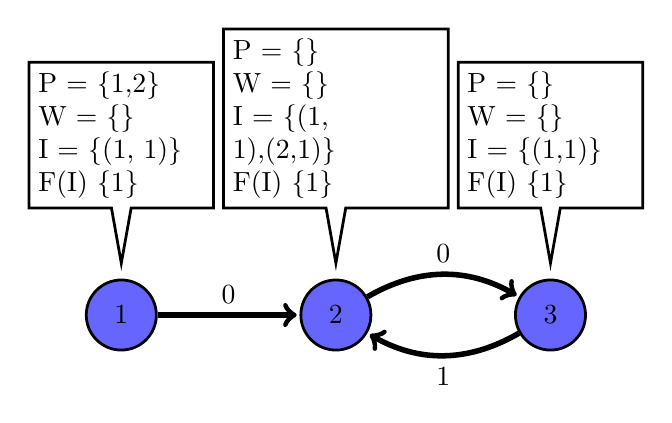
\begin{tikzpicture}[node distance = 1.8cm, auto]


\tikzstyle{operator} = [circle, draw, fill=blue!60, text width=1.5em, text centered, line width=1pt]

    \node [operator] at (0, 0) (1) {1};
    \node[draw, rectangle callout, above = of 1, line width=1pt, text width=6em, callout relative pointer={(0cm,-0.7cm)},above= 25pt] 
   { 
     P = \{1,2\}\\
     W = \{\}\\
     I = \{(1, 1)\}\\
     F(I) \{1\}
    };

    \node [operator, right = of 1] (2) {2};
     \node[draw, rectangle callout, above = of 2, line width=1pt, text width=7.45em, callout relative pointer={(0cm,-0.7cm)},above= 25pt] 
   { 
     P = \{\}\\
     W = \{\}\\
     I = \{(1, 1),(2,1)\}\\
     F(I) \{1\}
    };

    \node [operator, right = of 2] (3) {3}; 
     \node[draw, rectangle callout, above = of 3, line width=1pt, text width=6em, callout relative pointer={(0cm,-0.7cm)},above= 25pt] 
   { 
     P = \{\}\\
     W = \{\}\\
     I = \{(1,1)\}\\
     F(I) \{1\}
    };


    \draw [thick,->,shorten >=1pt, line width=2pt] (1) edge node {0} (2); 
    \draw [thick,->,shorten >=1pt, line width=2pt] (2) edge  [bend left]  node {0} (3);
     \draw [thick,->,shorten >=1pt, line width=2pt] (3) edge  [bend left]  node {1} (2); 


\end{tikzpicture}

  \end{center}
\end{frame}

\begin{frame}[fragile, noframenumbering]
  \frametitle{Local Propagation Example}
  \begin{center}
    \usetikzlibrary{shapes,arrows}
\usetikzlibrary{positioning}
\usetikzlibrary{calc,shapes.callouts,shapes.arrows}

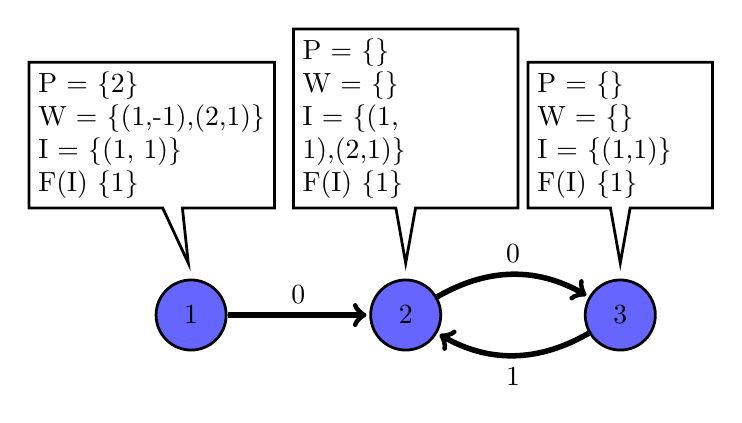
\begin{tikzpicture}[node distance = 1.8cm, auto]


\tikzstyle{operator} = [circle, draw, fill=blue!60, text width=1.5em, text centered, line width=1pt]

    \node [operator] at (0, 0) (1) {1};
    \node[draw, rectangle callout, above = of 1, line width=1pt, text width=8.2em, callout relative pointer={(0.2cm,-0.7cm)},above= 25pt, shift={(-0.5,0)}] 
   { 
     P = \{2\}\\
     W = \{(1,-1),(2,1)\}\\
     I = \{(1, 1)\}\\
     F(I) \{1\}
    };

    \node [operator, right = of 1] (2) {2};
     \node[draw, rectangle callout, above = of 2, line width=1pt, text width=7.45em, callout relative pointer={(0cm,-0.7cm)},above= 25pt] 
   { 
     P = \{\}\\
     W = \{\}\\
     I = \{(1, 1),(2,1)\}\\
     F(I) \{1\}
    };

    \node [operator, right = of 2] (3) {3}; 
     \node[draw, rectangle callout, above = of 3, line width=1pt, text width=6em, callout relative pointer={(0cm,-0.7cm)},above= 25pt] 
   { 
     P = \{\}\\
     W = \{\}\\
     I = \{(1,1)\}\\
     F(I) \{1\}
    };


    \draw [thick,->,shorten >=1pt, line width=2pt] (1) edge node {0} (2); 
    \draw [thick,->,shorten >=1pt, line width=2pt] (2) edge  [bend left]  node {0} (3);
     \draw [thick,->,shorten >=1pt, line width=2pt] (3) edge  [bend left]  node {1} (2); 


\end{tikzpicture}

  \end{center}
\end{frame}

\begin{frame}[fragile, noframenumbering]
  \frametitle{Local Propagation Example}
  \begin{center}
    \usetikzlibrary{shapes,arrows}
\usetikzlibrary{positioning}
\usetikzlibrary{calc,shapes.callouts,shapes.arrows}

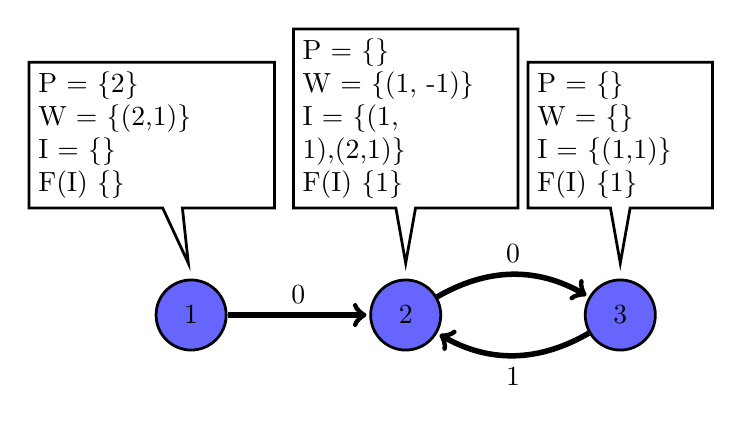
\begin{tikzpicture}[node distance = 1.8cm, auto]


\tikzstyle{operator} = [circle, draw, fill=blue!60, text width=1.5em, text centered, line width=1pt]

    \node [operator] at (0, 0) (1) {1};
    \node[draw, rectangle callout, above = of 1, line width=1pt, text width=8.2em, callout relative pointer={(0.2cm,-0.7cm)},above= 25pt, shift={(-0.5,0)}] 
   { 
     P = \{2\}\\
     W = \{(2,1)\}\\
     I = \{\}\\
     F(I) \{\}
    };

    \node [operator, right = of 1] (2) {2};
     \node[draw, rectangle callout, above = of 2, line width=1pt, text width=7.45em, callout relative pointer={(0cm,-0.7cm)},above= 25pt] 
   { 
     P = \{\}\\
     W = \{(1, -1)\}\\
     I = \{(1, 1),(2,1)\}\\
     F(I) \{1\}
    };

    \node [operator, right = of 2] (3) {3}; 
     \node[draw, rectangle callout, above = of 3, line width=1pt, text width=6em, callout relative pointer={(0cm,-0.7cm)},above= 25pt] 
   { 
     P = \{\}\\
     W = \{\}\\
     I = \{(1,1)\}\\
     F(I) \{1\}
    };


    \draw [thick,->,shorten >=1pt, line width=2pt] (1) edge node {0} (2); 
    \draw [thick,->,shorten >=1pt, line width=2pt] (2) edge  [bend left]  node {0} (3);
     \draw [thick,->,shorten >=1pt, line width=2pt] (3) edge  [bend left]  node {1} (2); 


\end{tikzpicture}

  \end{center}
\end{frame}

\begin{frame}[fragile, noframenumbering]
  \frametitle{Local Propagation Example}
  \begin{center}
    \usetikzlibrary{shapes,arrows}
\usetikzlibrary{positioning}
\usetikzlibrary{calc,shapes.callouts,shapes.arrows}

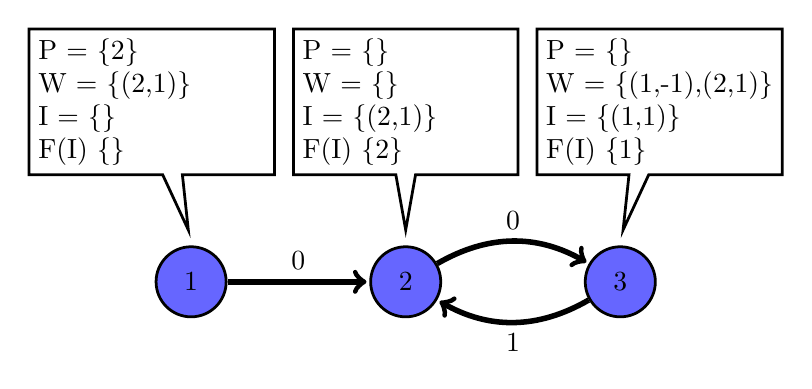
\begin{tikzpicture}[node distance = 1.8cm, auto]


\tikzstyle{operator} = [circle, draw, fill=blue!60, text width=1.5em, text centered, line width=1pt]

    \node [operator] at (0, 0) (1) {1};
    \node[draw, rectangle callout, above = of 1, line width=1pt, text width=8.2em, callout relative pointer={(0.2cm,-0.7cm)},above= 25pt, shift={(-0.5,0)}] 
   { 
     P = \{2\}\\
     W = \{(2,1)\}\\
     I = \{\}\\
     F(I) \{\}
    };

    \node [operator, right = of 1] (2) {2};
     \node[draw, rectangle callout, above = of 2, line width=1pt, text width=7.45em, callout relative pointer={(0cm,-0.7cm)},above= 25pt] 
   { 
     P = \{\}\\
     W = \{\}\\
     I = \{(2,1)\}\\
     F(I) \{2\}
    };

    \node [operator, right = of 2] (3) {3}; 
     \node[draw, rectangle callout, above = of 3, line width=1pt, text width=8.2em, callout relative pointer={(-0.2cm,-0.7cm)},above= 25pt, shift={(0.5,0)}] 
   { 
     P = \{\}\\
     W = \{(1,-1),(2,1)\}\\
     I = \{(1,1)\}\\
     F(I) \{1\}
    };


    \draw [thick,->,shorten >=1pt, line width=2pt] (1) edge node {0} (2); 
    \draw [thick,->,shorten >=1pt, line width=2pt] (2) edge  [bend left]  node {0} (3);
     \draw [thick,->,shorten >=1pt, line width=2pt] (3) edge  [bend left]  node {1} (2); 


\end{tikzpicture}

  \end{center}
\end{frame}

\begin{frame}[fragile, noframenumbering]
  \frametitle{Local Propagation Example}
  \begin{center}
    \usetikzlibrary{shapes,arrows}
\usetikzlibrary{positioning}
\usetikzlibrary{calc,shapes.callouts,shapes.arrows}

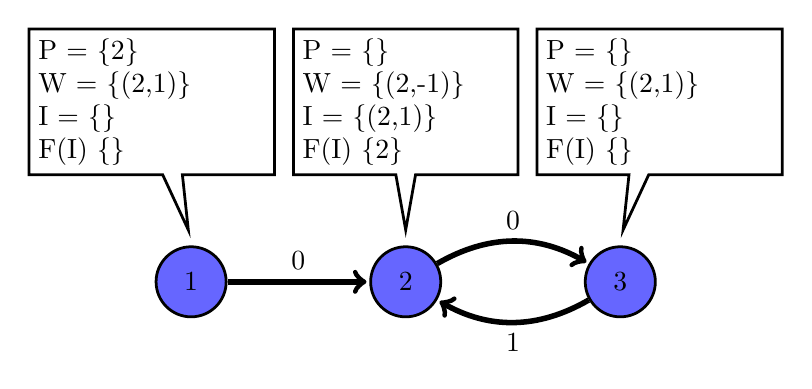
\begin{tikzpicture}[node distance = 1.8cm, auto]


\tikzstyle{operator} = [circle, draw, fill=blue!60, text width=1.5em, text centered, line width=1pt]

    \node [operator] at (0, 0) (1) {1};
    \node[draw, rectangle callout, above = of 1, line width=1pt, text width=8.2em, callout relative pointer={(0.2cm,-0.7cm)},above= 25pt, shift={(-0.5,0)}] 
   { 
     P = \{2\}\\
     W = \{(2,1)\}\\
     I = \{\}\\
     F(I) \{\}
    };

    \node [operator, right = of 1] (2) {2};
     \node[draw, rectangle callout, above = of 2, line width=1pt, text width=7.45em, callout relative pointer={(0cm,-0.7cm)},above= 25pt] 
   { 
     P = \{\}\\
     W = \{(2,-1)\}\\
     I = \{(2,1)\}\\
     F(I) \{2\}
    };

    \node [operator, right = of 2] (3) {3}; 
     \node[draw, rectangle callout, above = of 3, line width=1pt, text width=8.2em, callout relative pointer={(-0.2cm,-0.7cm)},above= 25pt, shift={(0.5,0)}] 
   { 
     P = \{\}\\
     W = \{(2,1)\}\\
     I = \{\}\\
     F(I) \{\}
    };


    \draw [thick,->,shorten >=1pt, line width=2pt] (1) edge node {0} (2); 
    \draw [thick,->,shorten >=1pt, line width=2pt] (2) edge  [bend left]  node {0} (3);
     \draw [thick,->,shorten >=1pt, line width=2pt] (3) edge  [bend left]  node {1} (2); 


\end{tikzpicture}

  \end{center}
\end{frame}

\begin{frame}[fragile, noframenumbering]
  \frametitle{Local Propagation Example}
  \begin{center}
    \usetikzlibrary{shapes,arrows}
\usetikzlibrary{positioning}
\usetikzlibrary{calc,shapes.callouts,shapes.arrows}

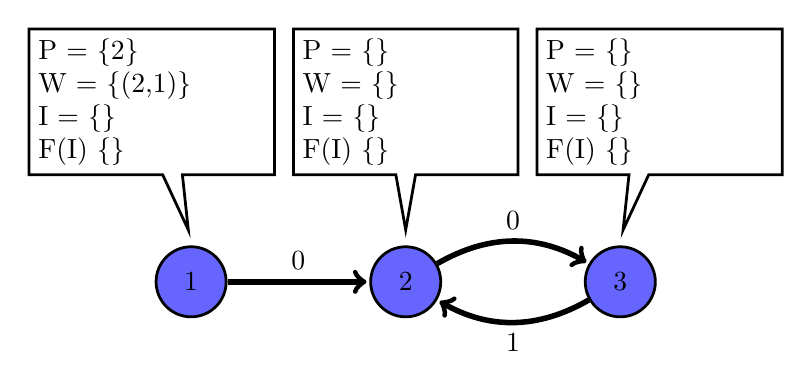
\begin{tikzpicture}[node distance = 1.8cm, auto]


\tikzstyle{operator} = [circle, draw, fill=blue!60, text width=1.5em, text centered, line width=1pt]

    \node [operator] at (0, 0) (1) {1};
    \node[draw, rectangle callout, above = of 1, line width=1pt, text width=8.2em, callout relative pointer={(0.2cm,-0.7cm)},above= 25pt, shift={(-0.5,0)}] 
   { 
     P = \{2\}\\
     W = \{(2,1)\}\\
     I = \{\}\\
     F(I) \{\}
    };

    \node [operator, right = of 1] (2) {2};
     \node[draw, rectangle callout, above = of 2, line width=1pt, text width=7.45em, callout relative pointer={(0cm,-0.7cm)},above= 25pt] 
   { 
     P = \{\}\\
     W = \{\}\\
     I = \{\}\\
     F(I) \{\}
    };

    \node [operator, right = of 2] (3) {3}; 
     \node[draw, rectangle callout, above = of 3, line width=1pt, text width=8.2em, callout relative pointer={(-0.2cm,-0.7cm)},above= 25pt, shift={(0.5,0)}] 
   { 
     P = \{\}\\
     W = \{\}\\
     I = \{\}\\
     F(I) \{\}
    };


    \draw [thick,->,shorten >=1pt, line width=2pt] (1) edge node {0} (2); 
    \draw [thick,->,shorten >=1pt, line width=2pt] (2) edge  [bend left]  node {0} (3);
     \draw [thick,->,shorten >=1pt, line width=2pt] (3) edge  [bend left]  node {1} (2); 


\end{tikzpicture}

  \end{center}
\end{frame}

\section{Verified Progress Tracking}

\begin{frame}
  \frametitle{Abadi et al.’s exchange protocol}
  \begin{columns}
    \begin{column}{.45\textwidth}
      \begin{itemize}
        \item Exchange Protocol Verification:
              \begin{itemize}
                \item Presented by Abadi et al. in TLA+
              \end{itemize}
              \pause
      \end{itemize}
      \begin{block}{Distribute \textbf{Safety}}
        If a timestamp is vacant in one worker (now), then that timestamp and any lesser it is vacant for the global system state (now and forever)
      \end{block}
    \end{column}
    \begin{column}{.45\textwidth}
      \begin{figure}
        \shadowbox{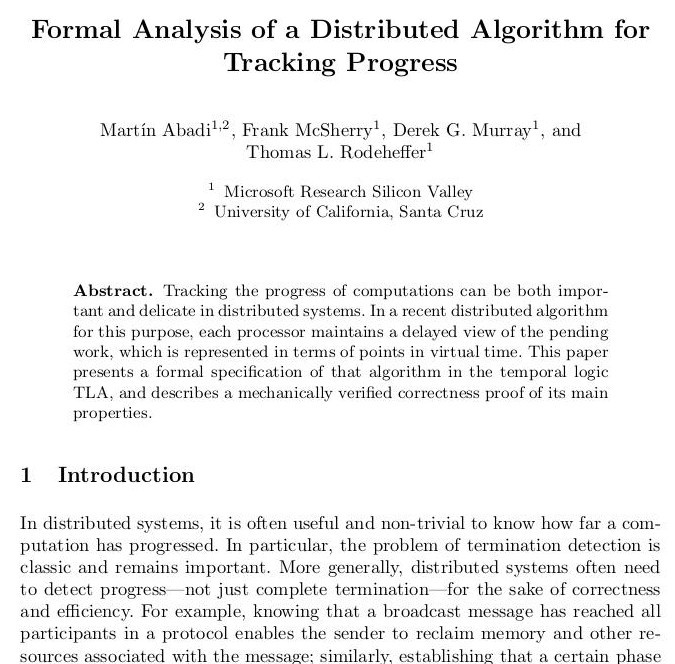
\includegraphics[width=0.95\textwidth]{tla+.jpg}}
      \end{figure}
    \end{column}
  \end{columns}
\end{frame}

\begin{frame}
  \frametitle{Verified Progress Tracking for Timely Dataflow}
  \begin{columns}
    \begin{column}{.45\textwidth}
      \begin{itemize}
        \item Exchange Protocol Verification:
              \begin{itemize}
                \item Refined version
                \item Same safety property
              \end{itemize}
              \pause
        \item Local Propagation Verification
      \end{itemize}
      \begin{block}{Local \textbf{Safety}}
        If all worklists neither contain timestamp $t$ nor smaller timestamps, then all locations know whether they may encounter $t$ in the future.
      \end{block}
    \end{column}
    \begin{column}{.45\textwidth}
      \begin{figure}
        \shadowbox{
\includegraphics[width=0.95\textwidth]{isabelle.jpg}}
      \end{figure}
    \end{column}
  \end{columns}
\end{frame}

\section{Verified Timely Dataflow}

\begin{frame}
  \frametitle{Verified Timely Dataflow}
  \begin{block}{General goal}
    Contribute to an ongoing formalization effort using the Isabelle proof assistant towards the first formally verified system for the analysis of big data.
  \end{block}
  \pause
  \begin{block}{Specific goals}
    \begin{enumerate}
      \item Termination of the propagation protocol
      \item Executable Progress Tracking Protocol
      \item Data plane
      \item Scopes
      \item DSL
      \item Experiments
    \end{enumerate}
  \end{block}
\end{frame}

\begin{frame}
  \frametitle{Termination of the propagation protocol}
  \begin{itemize}
    \item \textit{propagate} is a relation between two system configurations and also parameterized by location and a timestamp:
          \begin{itemize}
            \item Propagating the timestamp \textit{t} in location \textit{loc} the configuration \textit{c1} turns into \textit{c2}
          \end{itemize}
    \item We aim to show that it's impossible cannot propagate forever
    \item We've already managed to show that for a fixed timestamp it cannot be propagate forever
  \end{itemize}
\end{frame}

\begin{frame}
  \frametitle{Executable Progress Tracking Protocol}
  \begin{itemize}
    \item The propagation protocol is already executable (Sara Decova's master thesis)
    \item The Exchange protocol also should be made executable
          \begin{itemize}
            \item Prove that the functions are consistent with the relational counterparties
          \end{itemize}
  \end{itemize}
\end{frame}

\begin{frame}
  \frametitle{Data plane}
  \begin{itemize}
    \item Nodes must be real operators: they execute user defined functions over the data
    \item Edges must be channels: they are streams with push and pull API
          \begin{itemize}
            \item Must exchange data between different workers
          \end{itemize}
    \item Low level operator constructors (define operators for any amount of inputs and outputs)
    \item A set of generally useful built-in operators: filter, filter partition, count, aggregate, etc
    \item The Safety properties again!
          \begin{itemize}
            \item Use safety to show properties of operators and dataflows
                  \begin{itemize}
                    \item Ex: show that \textit{count} doesn't mix the results of different (comparable) timestamps
                  \end{itemize}
          \end{itemize}
    \item Executable from the start
  \end{itemize}
\end{frame}

\begin{frame}
  \frametitle{Scopes}
  \begin{itemize}
    \item Hierarchal dataflows: an operator can also be a sub-dataflow inside of a dataflow
    \item This is designed as scopes
          \begin{itemize}
            \item An additional timestamp dimension
          \end{itemize}
    \item Another propagation (upwards and downwards)
    \item The Safety properties once again!
  \end{itemize}
\end{frame}

\begin{frame}
  \frametitle{DSL}
  \begin{itemize}
    \item Writting dataflow programs in Isabelle is quite inconvenient
    \item A suitable domain-specific language (DSL)
  \end{itemize}
\end{frame}

\begin{frame}
  \frametitle{Experiments}
  \begin{enumerate}
    \item How faithful is the verified model to the Rust implementation?
    \item Are there any bugs in the Rust implementation not present in the verified code?
    \item How does the performance of the verified code compares to the Rust implementation?
  \end{enumerate}
\end{frame}

\section{Questions, comments and suggestions}

\end{document}
